\section{Results}
\label{sec:Res}

% ----------------------------------------------------------------------- %
% ----------------------------------------------------------------------- %
\subsection{General estimation results}
\label{sec:feasest}

An application of the SRS, \psmall{} and \extpsynth{} estimator was not feasible for 17 of all 405 FR-units due to an insufficient terrestrial sample size of $n_{2,G} < 2$. We further restricted the calculation of the \psmall{} and \extpsynth{} estimator to small area units with a minimum terrestrial sample size of $n_{2,G} \geq 4$ to avoid unstable estimates. This affected 65 additional FR units and limited unbiased two-phase estimations to 321 (79\%) of the 405 FR units. It should be noted that also the \psynth{} estimator could not be applied for 2 FR-units since $n_{1,G} < 2$. Due to substantial larger sample sizes, all estimators could however be applied to all 45 FA units. The average value and the range of the mean timber volume estimates over the evaluated FA and FR units turned out to be very similar between all estimators (table \ref{tab:estres}). An additional pairwise comparison of the 95\% confidence intervals revealed that the four estimators did in fact not produce statistically different point estimates for all FA and FR units. This confirmed that the differences between the estimators are solely found in the precision which they provide for the point estimates.


%% NOTES
%
% Feasibility: 
% FA-level: for 44 out of 45 FA-units, the full model could be applied. For one remaining, only the model without tree species was applied.
% 
% FR-level: 
% o mathemat. feasibility:
%    - op-estimation feasible for 388 of the 405 fu-units. --> for 17 fus not possible due to n2G < 2
%    - psmall / extpsynth possible for 388 of the 405 units (for 17 fus not possible). Reason: n2G < 2 (identical with op)
%    - psynth not possible for 403 of 405. For 2 units not possible due to n1G < 2 (these two are included in the 19 above).
%    -> basically, for these 2 fu-units, none of the estimators could produce estimations due to n1G < 2
%  o restriction of unbiased estimtors to n2G >= 4: 
%    - psmall / extpsynth: 65 of the 386 fu-units have n2G < 4, so theyx cancel out. Thus we have 19 + 65 = 84 fu-units for which no psmall & extpsynth estimations were deliverable.
%       ==> Thus, we have unbiase estimations for 321 of 405 fu units (79%)

% Mention: a comparison of the confidence intervals between revealed that the 

\begin{table}[H]
	\begin{center}
		\caption{Descriptive summary of point estimates and estimation errors on the two forest district levels. $N_u$: number of evaluated small area units.}
		\vspace{0.2cm}
		\label{tab:estres}
		{\small %
			\begin{tabular}{c|l c|c c c|c c c} %8cols
				\hlineB{1}
				\multirow{2}{*}{District level} & \multicolumn{2}{c|}{\multirow{2}{*}{Estimator}} & \multicolumn{3}{c|}{Point estimates} & \multicolumn{3}{c}{Errors [\%]} \\
				\cline{4-9} & & & mean & min & max & mean & min & max \\
				\hline \hline
				\multirow{4}{*}{FA} & SRS       & ($N_u$=45)  & 300.16 & 215.91 & 392.84 &  6.69 & 3.87 & 13.21 \\
				                    & PSMALL    & ($N_u$=45)  & 307.29 & 209.26 & 417.10 &  5.16 & 3.46 & 14.33 \\
				                    & EXTPSYNTH & ($N_u$=45)  & 307.27 & 209.01 & 415.02 &  4.78 & 3.25 & 13.88 \\
				                    & PSYNTH    & ($N_u$=45)  & 306.90 & 223.51 & 409.92 &  2.34 & 1.54 &  3.95 \\
				\hlineB{2}          
				\multirow{4}{*}{FR} & SRS       & ($N_u$=388) & 301.83 &  99.89 & 612.13 & 18.32 & 0.34 & 104.97 \\
				                    & PSMALL    & ($N_u$=321) & 308.15 & 159.64 & 568.67 & 12.24 & 3.48 &  44.94 \\
				                    & EXTPSYNTH & ($N_u$=321) & 308.38 & 154.07 & 544.34 & 11.34 & 3.60 &  40.91 \\
				                    & PSYNTH    & ($N_u$=403) & 307.82 & 166.01 & 444.29 & 4.65  & 2.56 &  62.51 \\
				\hline \hline
			\end{tabular}
		}%
	\end{center}
\end{table}



% ----------------------------------------------------------------------- %
% ----------------------------------------------------------------------- %
\subsection{Estimation errors}
\label{sec:esterr}

On both small area levels, the design-unbiased estimators \psmall{} and \extpsynth{} led to a substantial reduction in the estimation errors compared to the SRS estimator (fig. \ref{fig:disterrors}). On the FA level, the SRS estimator yielded an estimation error of 6.7\% on average compared to 5.2\% and 4.8\% under the \extpsynth{} and \psmall{} estimator (table \ref{tab:estres}). The cumulative error distribution (fig. \ref{fig:disterrors}, left) reveals that under the SRS estimator, errors $\leq$ 5\% were achieved for 17\% of the FA units (8 of 45). This proportion could be increased to 62\% (28 FA units) and 73\% (33 FA units) by application of the \psmall{} and \extpsynth{} estimator. 95\% of all estimates exhibited errors $\leq$ 9.5\% under the SRS estimator and $\leq$ 6.6\% when using \psmall{} or \extpsynth{}. Estimation errors higher than 10\% only appeared twice for each of the three estimators.\par
The error reduction by the \psmall{} and \extpsynth{} estimator was even more pronounced on the FR level (fig. \ref{fig:disterrors}, right), although the overall error niveau was substantially higher than on FA level. The average error under the SRS estimator was 18.3\%, while it was 11.3\% and 12.2\% under the \psmall{} and \extpsynth{} estimator (table \ref{tab:estres}). Errors smaller than 10\% were achieved for 15\% of the FR units by the SRS estimator, and for 46\% by the \psmall{} and \psynth{} estimator. 95\% of the 321 FR units where \psmall{} and \extpsynth{} could be applied exhibited errors $\leq$ 20\%. In comparion, the SRS estimates resulted in errors $\leq$ 36.6\% for 95\% of the 388 FR units.

\begin{figure}[H]
	\centering
	\resizebox{1\hsize}{!}{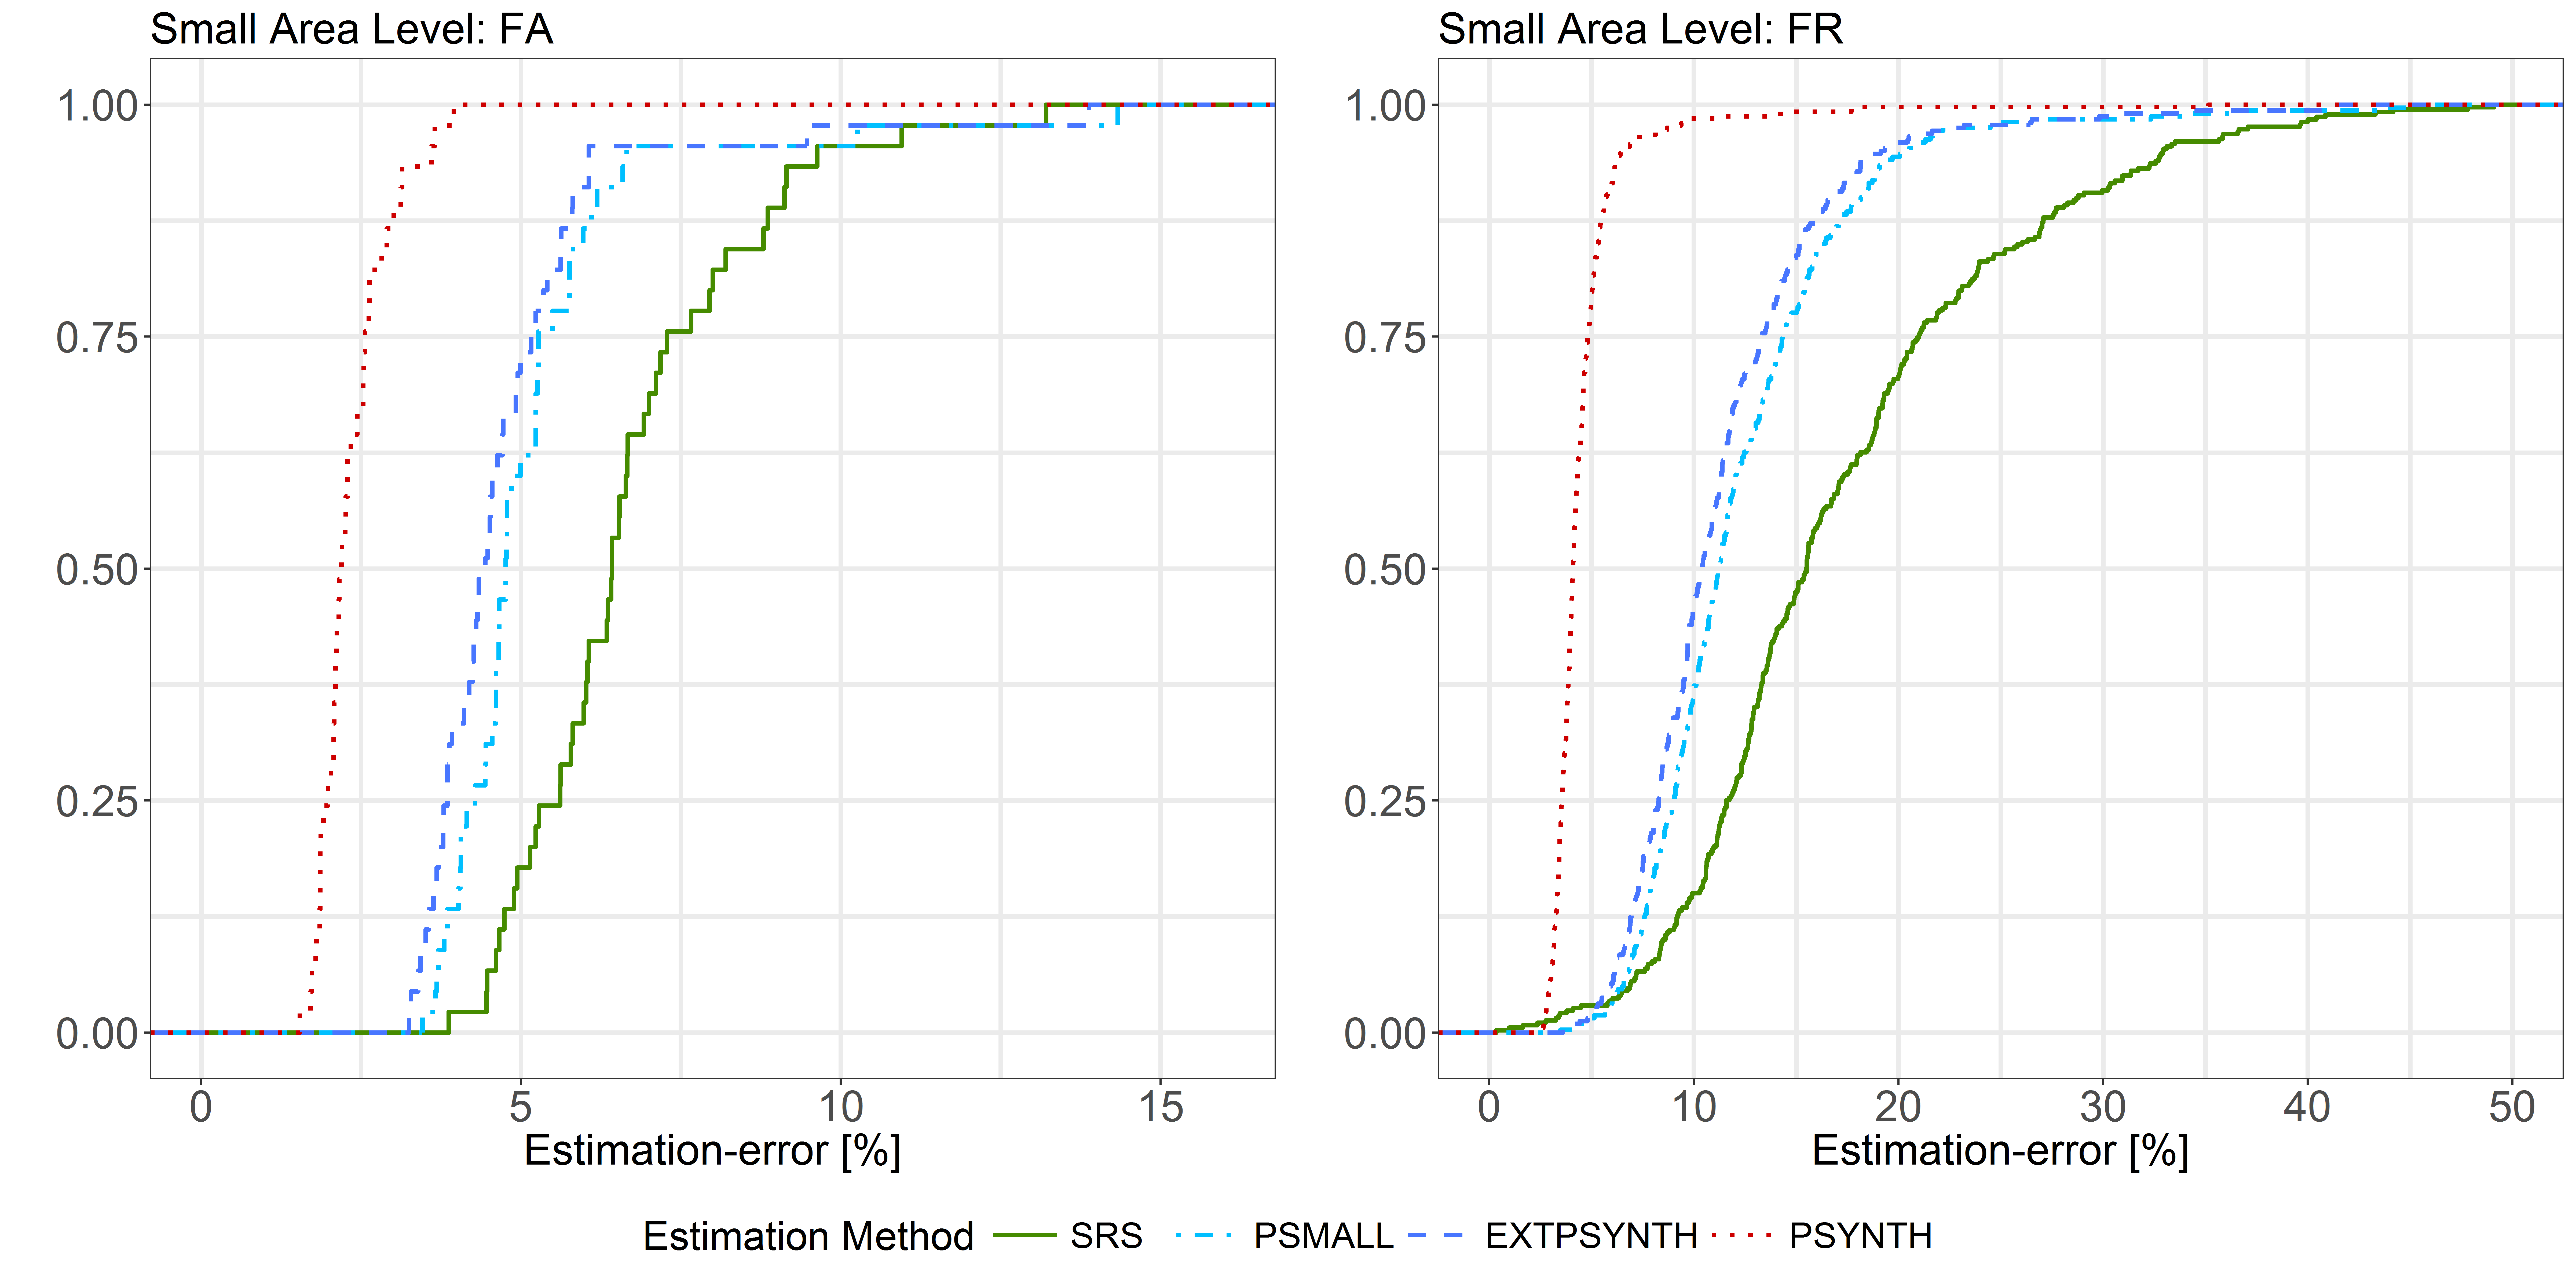
\includegraphics{fig/error_distr_foa_fu.png}}
	\caption{Cumulative distribution of estimation errors under the simple random sampling (SRS), the pseudo small (\psmall{}), the extended pseudo synthetic (\extpsynth{}) and the pseudo synthetic (\psynth{}) estimator. \textit{Left}: Results for the 45 FA units. \textit{Right}: Results for the 388 (SRS), 321 (\psmall{} / \extpsynth{}) and 403 (\psynth{}) FR units.}
	\label{fig:disterrors}
\end{figure}

On both small area levels, the \psynth{} estimator resulted in much smaller estimation errors compared to \psmall{} and \extpsynth{}. This was as expected, since the \psynth{} variance estimate does not take the residual variation in each small area unit into account (section \ref{sec:psynth}). Compared to the asymptotically design-unbiased estimators \psmall{} and \extpsynth{}, the estimation errors produced by \psynth{} thus seem to be too optimistic. One should also recall that the estimates of the \psynth{} estimator are potentially design-biased.

%% NOTES
 %Estimation errors smaller than 10\% were achieved for only 15\% (xx) of all FR units under SRS, while this proportion could be increased to 38\% and 46\% by PSMALL and EXTPSYNTH. 




% ----------------------------------------------------------------------- %
% ----------------------------------------------------------------------- %
\subsection{Comparison of \psmall{} and \extpsynth{}}
\label{sec:comp}

Figure \ref{fig:disterrors} reveals that the error distribution of \psmall{} and \extpsynth{} are very similar, with \psmall{} showing marginally higher estimation errors. In order to investigate the differences between \psmall{} and \extpsynth{}, we compared the g-weight variances of both estimators for all 321 FR units (fig. \ref{fig:compvar}, left). As obvious, \psmall{} yielded slightly larger variances for the vast majority of the estimates. As addressed in section \ref{sec:extpsynth}, one possible explanation for such differences was the effect of one or more cluster not entirely being included in a small area unit, as this would constitute a violation of the \extpsynth{} estimator. This violation was actually observed in 155 of the 321 FR units (48\%). However, the affected FR units (depicted in red diamonds, fig. \ref{fig:compvar}) did not show a significant divergence from the \psmall{} variances with respect to the remaining unaffected FR units. The variance differences between the two estimators were thus due to the mathematical formulations of the \psmall{} and \extpsynth{} estimator, which are asymptotically equivalent only under large terrestrial sample sizes $n_{2,G}$ within the small area \citep[pp.17--18]{mandallaz2016}. An additional comparison of the absolute differences in the g-weight variance (fig. \ref{fig:compvar}, right) revealed that large divergences did in fact particularly occur for small area units with small terrestrial sample sizes ($n_{2,G} \leq 5$). The differences decreased with increasing sample size and thus confirmed the asymptotic relationship between the two estimators. However, a comparison of the confidence intervals of \psmall{} and \extpsynth{} revealed that the variance differences did not lead to statistically significant point estimates. The results indicate that the adjustment of the intercept term to the data within a small area used in the \extpsynth{} estimator will in general yield slightly smaller variances than the \psmall{} estimator.\par



% NOTES:
% - Section \ref{sec:comp} provides a more detailed analysis of the differences between the two estimators.
% - DM-explanation: The model residuals and thus the residual variance for extpsynth should in general be a bit better than those of psmall, since we additionally adjust the regression
%                   to the small area data by introducing the sae-indicator variable (even if this is strictly speaken only a means to cause zero-mean-residuals)
%                   ==> we even can relate the differences to the residual variation, since the first and second term of extpsynth and psmall area identical with exception 
%                       of the adjusted regression coefficient
% - we can see the asymptotic of psmall and extpsynth: with increasing n2G, psmall and extpsynth are mathematically identical
% ==> so differences will particularly concern sae units with small n2G (threshold seems to be around n2G < 10)
%
% for Discussion:
% - our analyses 
%   a) suggest that the differences between \psmall{} and \extpsynth{} become negligible for sample sizes $n_{2,G}$ larger than 10 due to the asymptotic relationship between these estimators 
%   b) showed that violation of the '\extpsynth{}'-assumption had only minor effects on the variance estimates that did not lead to statistically different point estimates 
%   c) indicate that \extpsynth{} will in general have slightly smaller est.variances due to a slightly better model fit through the data in the small area, which is caused by the 
%      adjusted intercept (which however is mainly a means to insure the zero-mean-residual assumption in the \extpsynth{}-estimator


\begin{figure}[H]
	\centering
	\resizebox{1\hsize}{!}{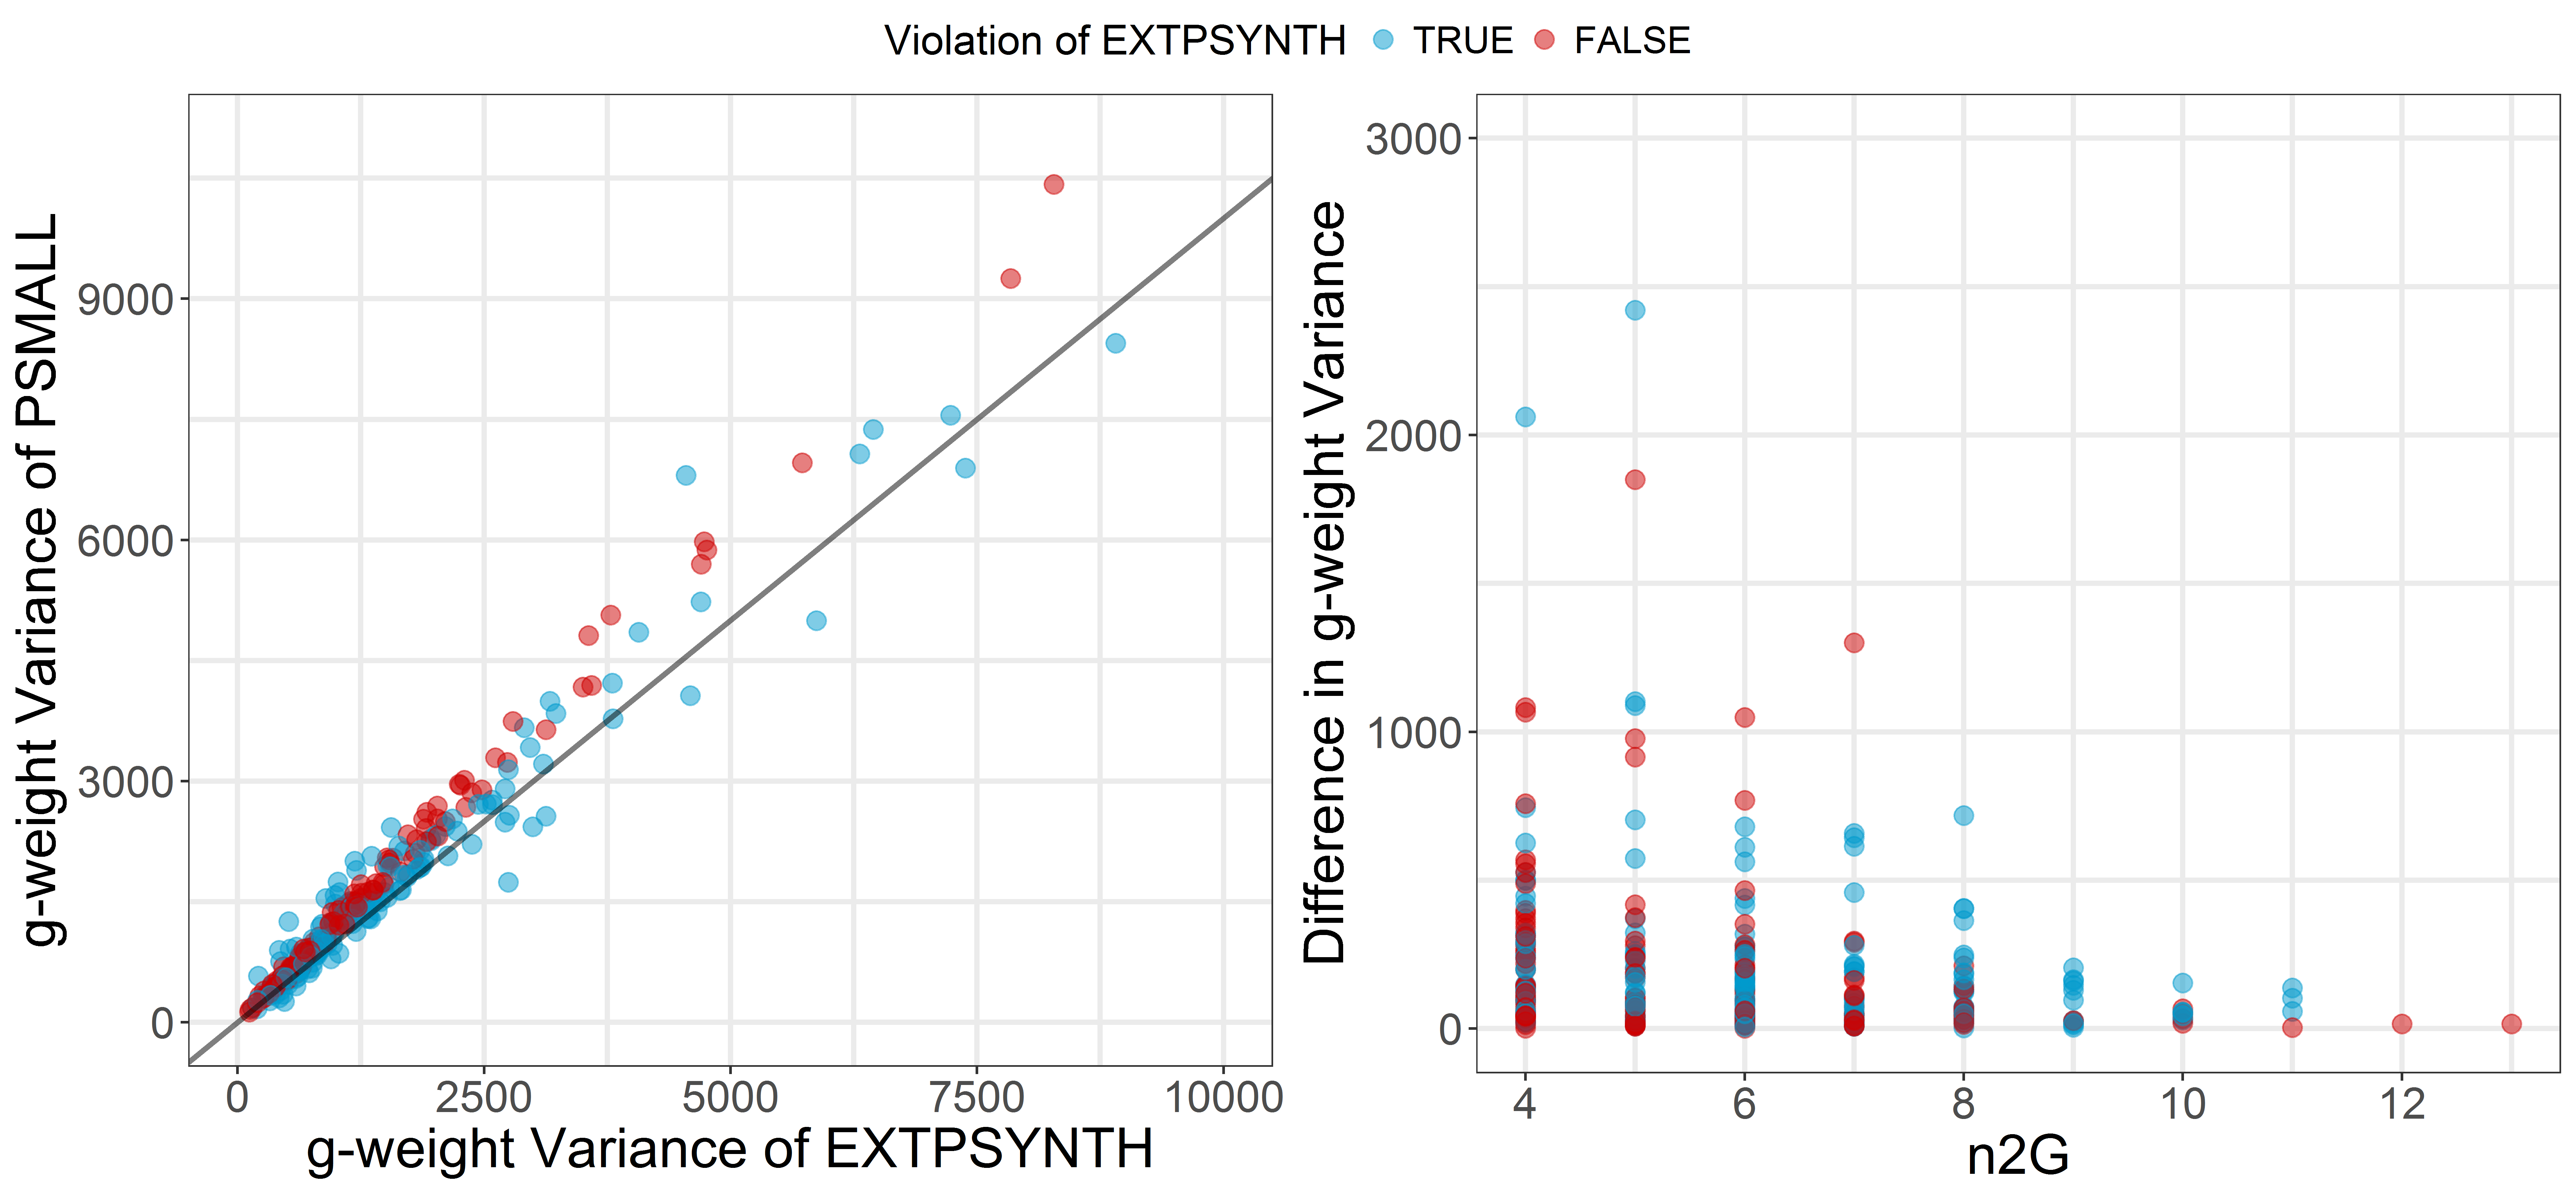
\includegraphics{fig/psmall_vs_extpsynth_fu.png}}
	\caption{\textit{Left}: Comparison of the g-weight variance between the PSMALL and the EXTPSYNTH estimator for the 321 FR units.
		\textit{Right}: Difference in g-weight variance between the PSMALL and the EXTPSYNTH estimator in dependence of the terrestrial data ($n2G$) in the FR unit.}
	\label{fig:compvar}
\end{figure}




% ----------------------------------------------------------------------- %
% ----------------------------------------------------------------------- %
\subsection{Reduction of SRS variance by \psmall{} and \extpsynth{}}
\label{sec:gain_eval}

A direct comparison of the realized variances within the small area units revealed that the application of the design-unbiased estimators (\psmall{} and \extpsynth{}) led to a reduction of the respective SRS variance in all FA units. In 75\% of the FA units, the \extpsynth{} estimator was able to reduce the SRS variance by up to 54.1\% (fig. \ref{fig:gain}). The reduction in variance was also expressed in the relative efficiency values, which were 2.02 on average and ranged between 1.18 and 4.13 on the FA level. On FR-level, the reduction in variance and the relative efficiencies reached even higher values (table \ref{tab:gain} and fig. \ref{fig:gain}). The \psmall{} estimator again yielded slightly lower variance reductions and relative efficiencies due to the generally smaller variances of the \extpsynth{} estimator (section \ref{sec:comp}).

\begin{figure}[H]
	\centering
	\resizebox{0.7\hsize}{!}{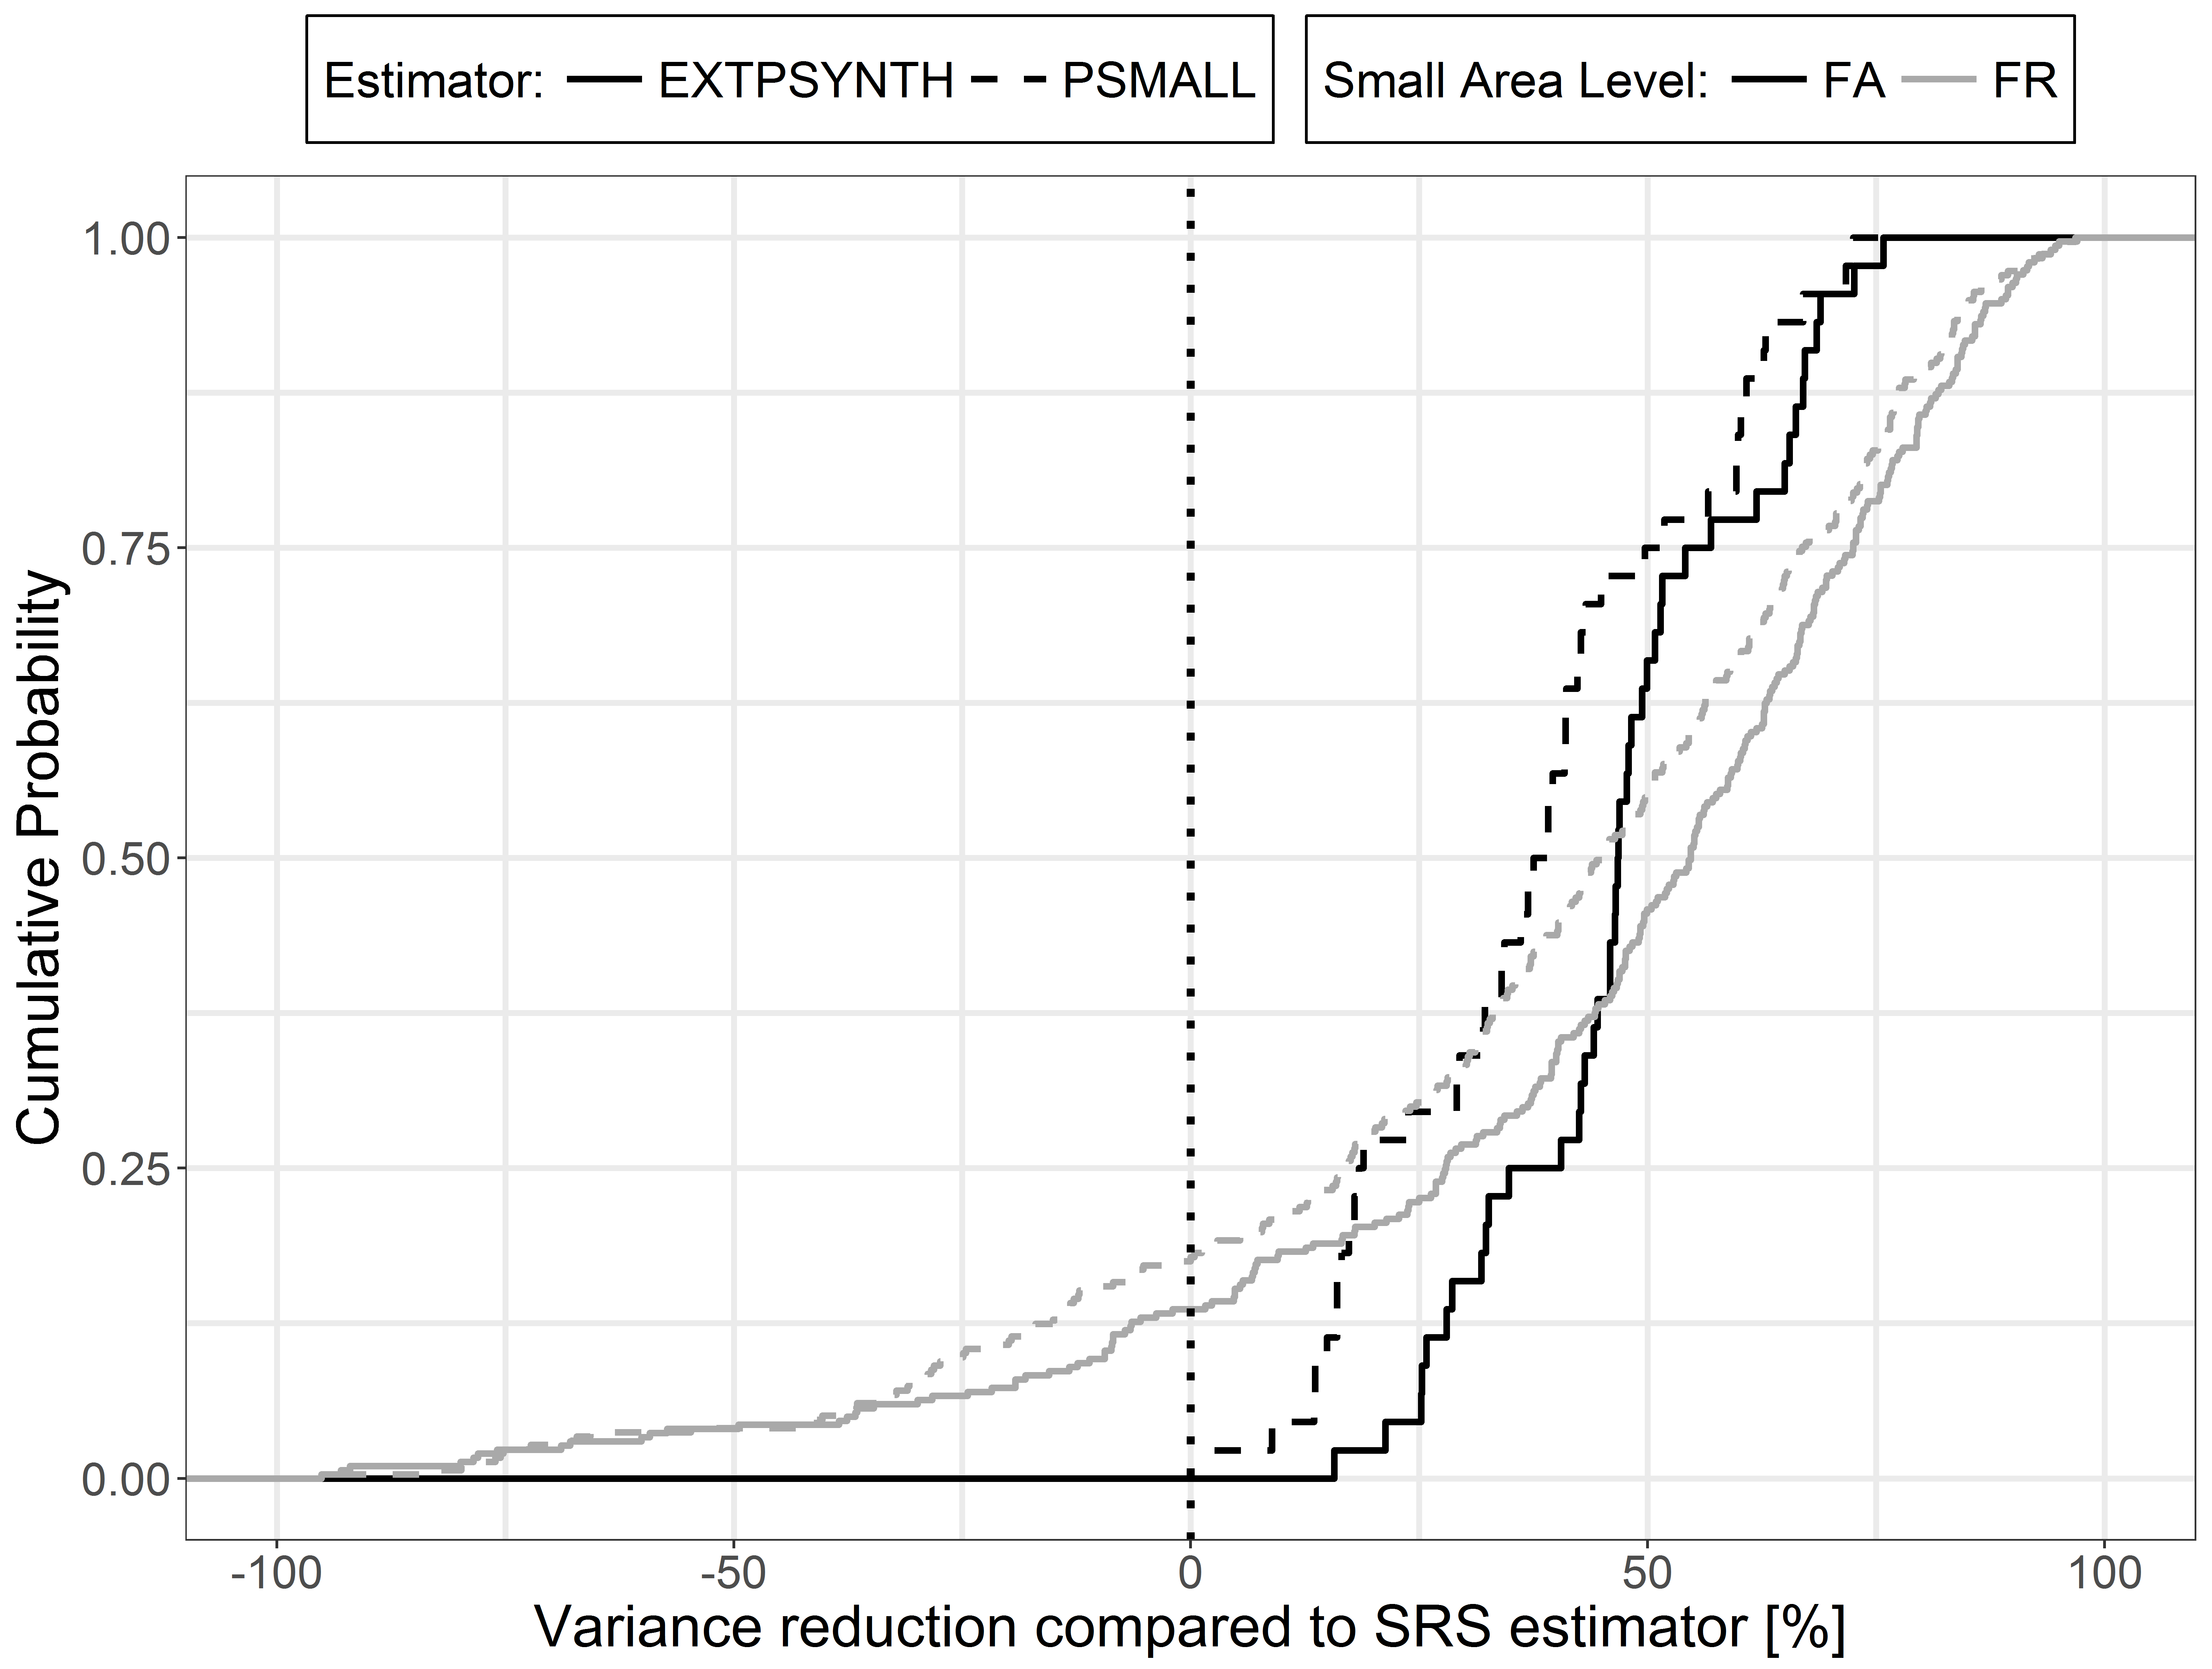
\includegraphics{fig/compare_onephase_extpsynth_psmall.png}}
	\caption{Cumulative distribution of variance reduction by the PSMALL and EXTPSYNTH compared to the SRS estimator for the  45 FA and 321 FR units.}
	\label{fig:gain}
\end{figure}

\begin{table}[H]
	\begin{center}
		\caption{Descriptive summary of SRS variance reduction and relative efficiencies on the two forest district levels. $N_u$: number of evaluated small area units.}
		\vspace{0.2cm}
		\label{tab:gain}
		{\small %
			\begin{tabular}{c|l c|c c c|c c c} %8cols
				\hlineB{1}
				\multirow{2}{*}{District level} & \multicolumn{2}{c|}{\multirow{2}{*}{Estimator}} & \multicolumn{3}{c|}{Reduction of SRS variance [\%]} & \multicolumn{3}{c}{relative efficiency} \\
				\cline{4-9} & & & mean & min & max & mean & min & max \\
				\hline \hline
				\multirow{2}{*}{FA} & PSMALL    & ($N_u$=45)  & 33.51 &  2.6 & 72.5 & 1.74 & 1.03 & 3.64 \\
				& EXTPSYNTH & ($N_u$=45)  & 43.30 & 15.7 & 75.8 & 2.03  & 1.18 & 4.13 \\
				\hlineB{2}          
				\multirow{2}{*}{FR} & PSMALL    & ($N_u$=321) & 12.48 & -1203.9 & 96.8 & 2.54 & 0.08 & 31.61  \\
				& EXTPSYNTH & ($N_u$=321) & 24.75 & -892.7  & 97.0 & 2.95 & 0.10 & 33.70 \\
				\hline \hline
			\end{tabular}
		}%
	\end{center}
\end{table}

However, cases also occurred on the FR level where one or both two-phase estimators produced larger variance values than under the SRS estimator. This particularly happened in 19\% (61) of the FR units under the \extpsynth{}, and in 24\% (76) of the FR units under the \psmall{} estimator. One possible reason for this was supposed to be a large residual variance due to a poor performance of the regression model within the small area unit. In order to investigate this hypothesis, we analyzed the three variance terms of the \psmall{} estimator (eq. \ref{eq:psmall_var}), i.e. the variance introduced by the uncertainty of the regression coefficients (term 1), the variance caused by estimating the auxiliary means (term 2), and the variance of the model residual (term 3).  The latter particularly expresses the model performance within the small area unit. Figure \ref{fig:fail} illustrates the percentage reduction or increase of the SRS variance when compared to the \psmall{} variance for all FR units in dependence on a) the impact of residual variance on the g-weight variance, and b) the terrestrial sample size $n_{2,G}$.\par

Obviously, the residual term generally constitutes the dominating part of the \psmall{} g-weight variance (around 84\% on average). However, a high proportion of the residual variance term seems not to be the driver for large \psmall{} variances, as apparent from Fig. \ref{fig:fail} (\textit{right}). The FR units where the \psmall{} estimator produced larger variances than the SRS estimator did not systematically differ from the majority of the FR units where \psmall{} performed better than SRS. However, FR units with exceptionally large variance increases compared to SRS particularly occurred under small terrestrial sample sizes of $n_{2,G} = 4$ (fig. \ref{fig:fail}, \textit{left}). These FR units exhibited a 272\% average increase of the SRS variance, compared to 62\% for the critical FR units with $n_{2,G} > 4$. In comparison, the achievable reduction in SRS variances compared to SRS were not considerably impacted by the terrestrial sample size (fig. \ref{fig:fail}, \textit{right}). The average reduction of these units was around 50\% under sampling sizes of both $n_{2,G} = 4$ and $n_{2,G} > 4$. 

\begin{figure}[H]
	\centering
	\resizebox{1\hsize}{!}{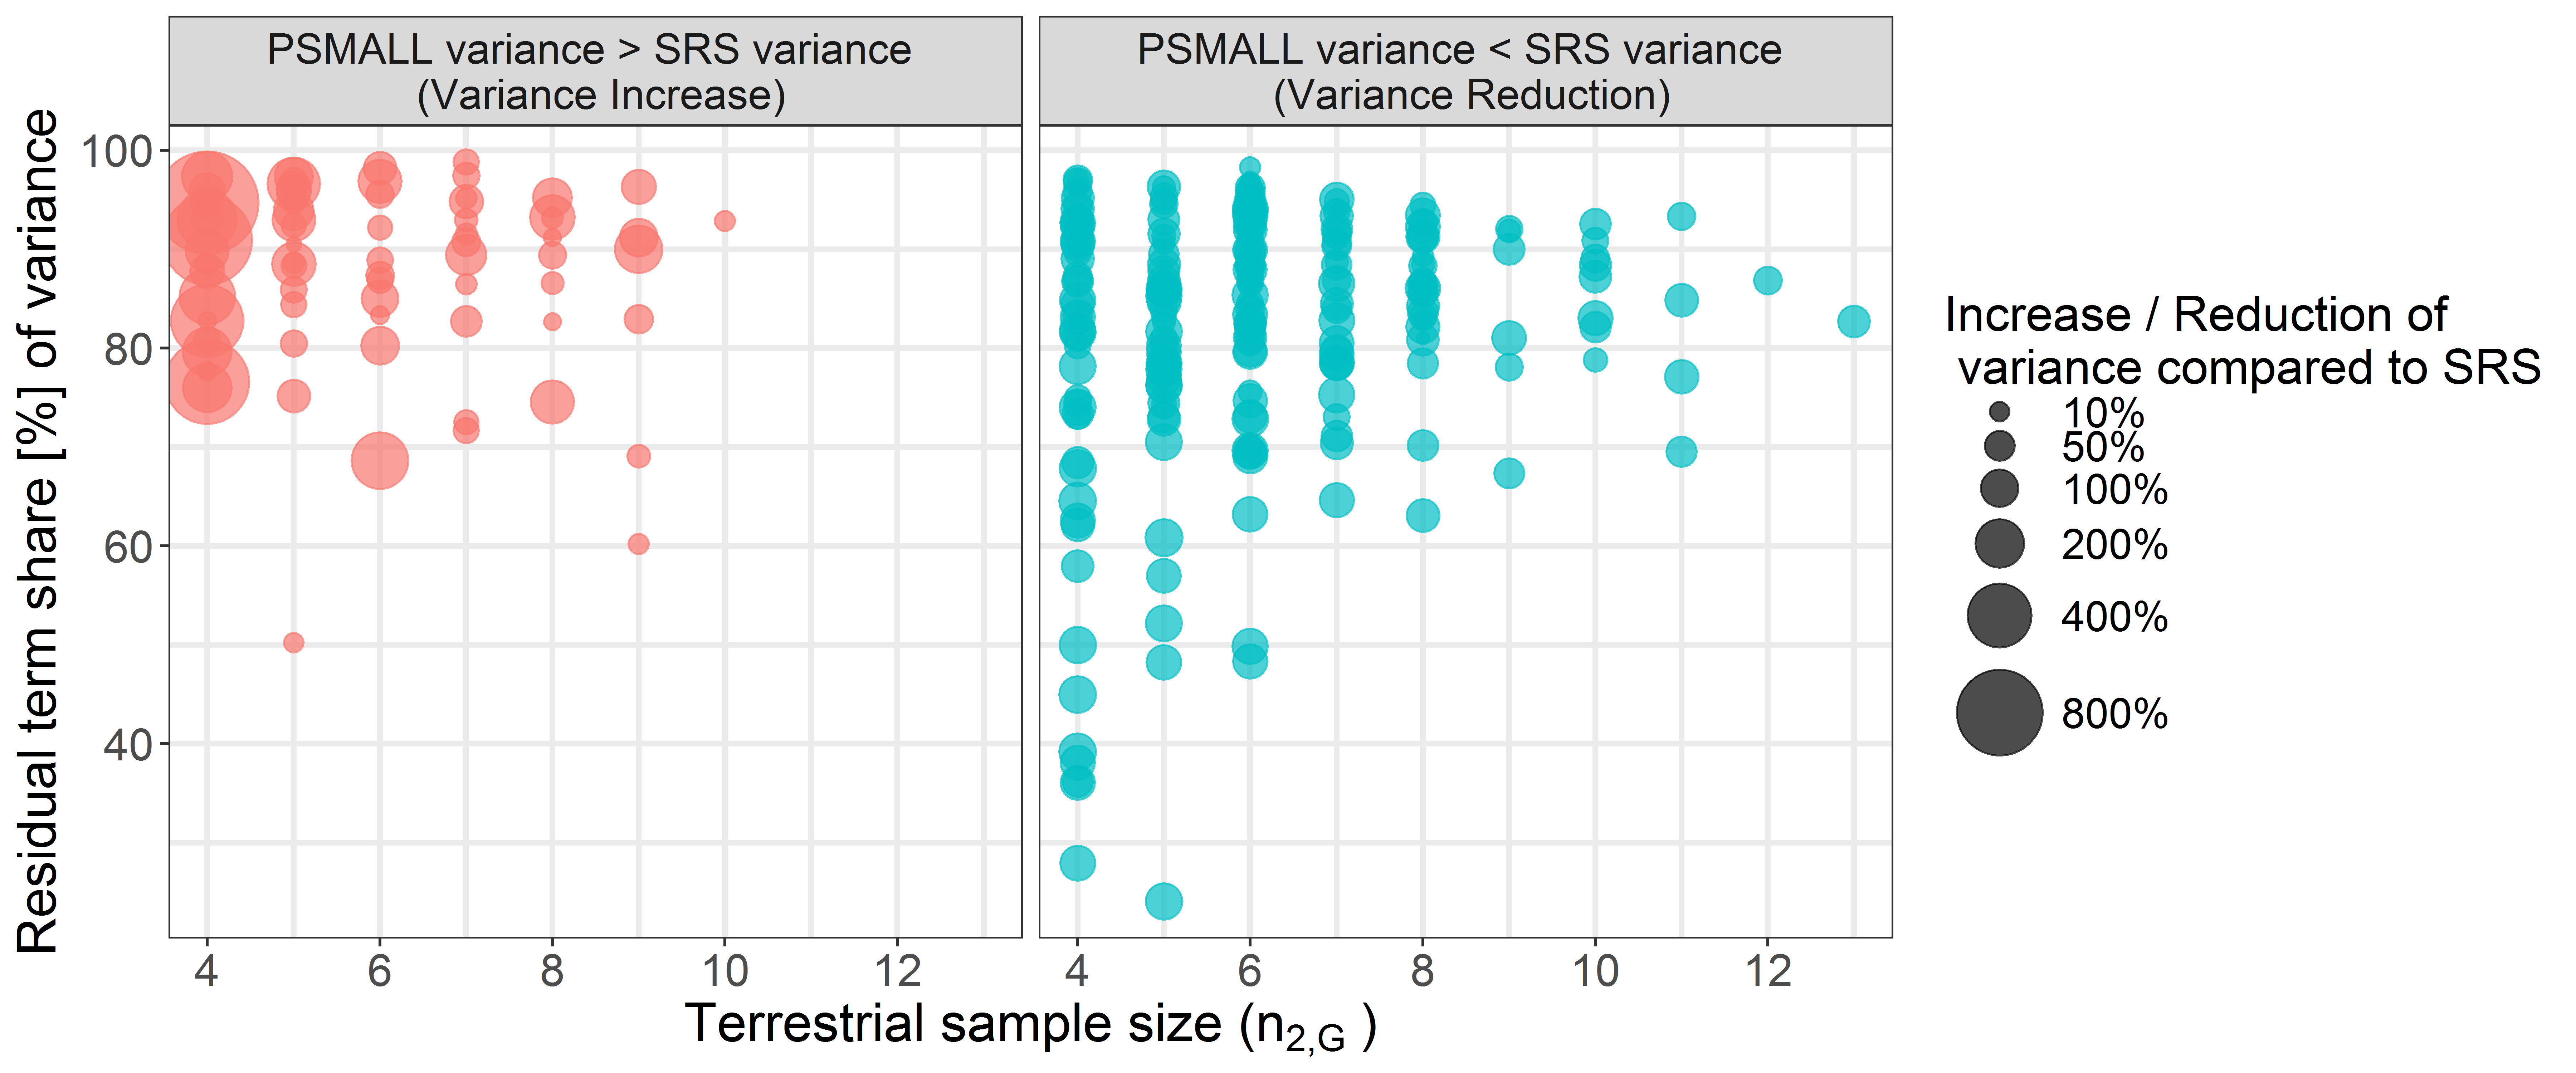
\includegraphics{fig/eval_2phase_fail_11.png}}
	\caption{}
	\label{fig:fail}
\end{figure}




% discussion: This also underlined why the \psynth{} estimator, which does not take the residual variation into account, produced substantially smaller variances than the design-unbiased estimator. 
% These findings suggest that moderate or poor model fits within a small area can cause the \psmall{} and \extpsynth{} estimator to produce higher variances than the SRS estimator particularly under small terrestrial sample sizes.



%\begin{figure}[H]
%	\centering
%	\resizebox{1\hsize}{!}{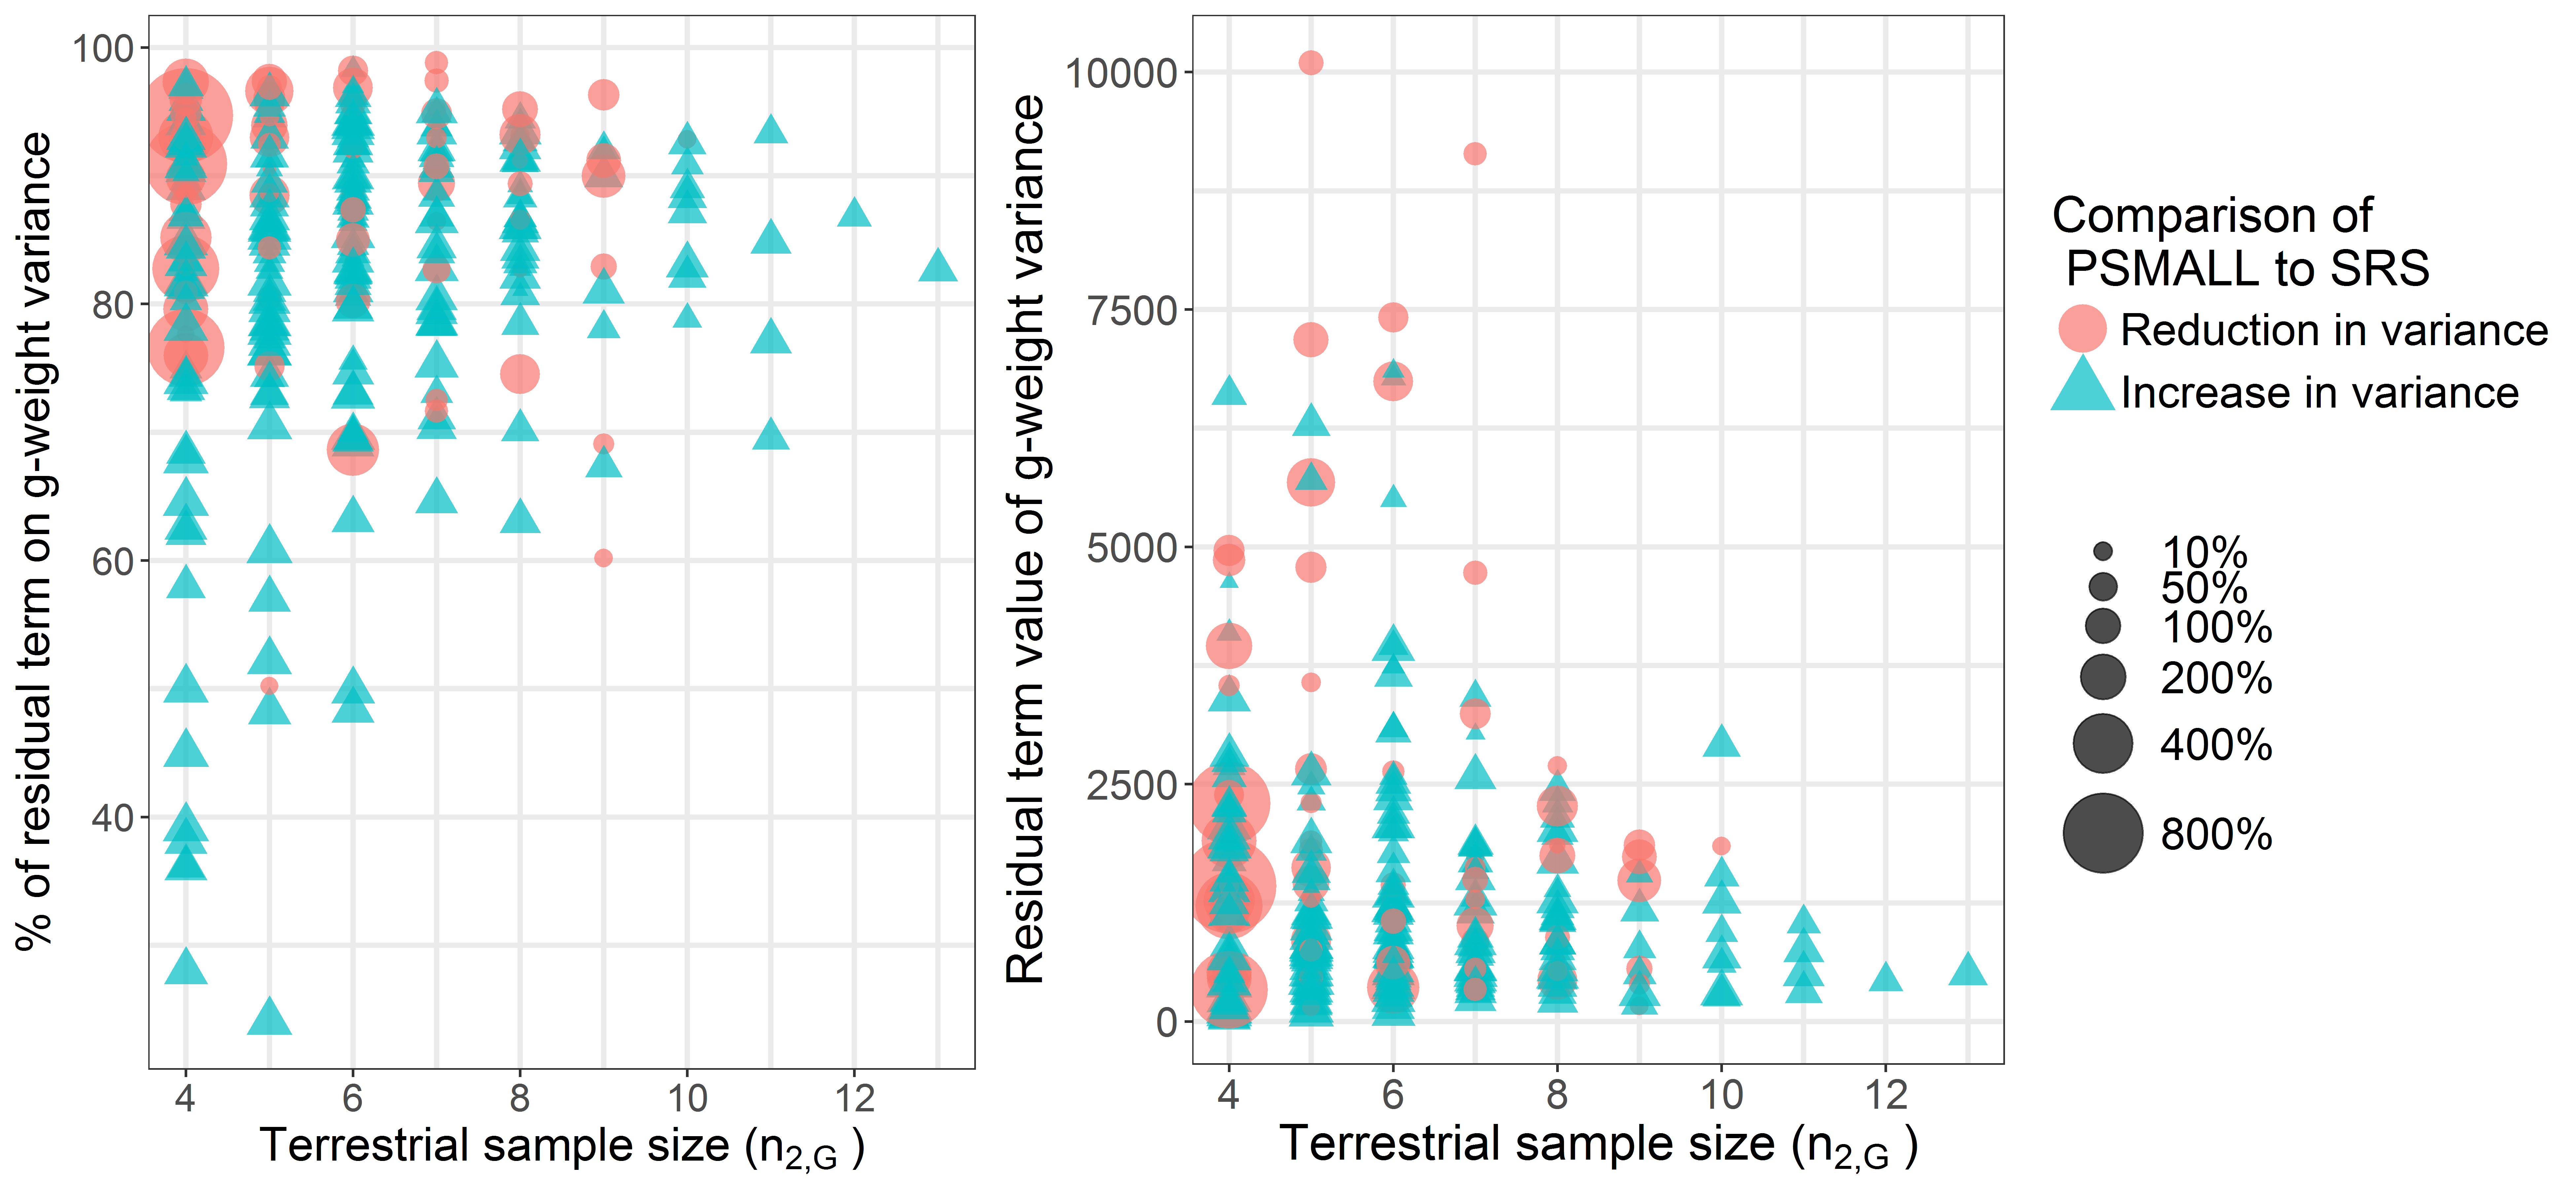
\includegraphics{fig/eval_2phase_fail.png}}
%	\caption{}
%	\label{fig:fail1}
%\end{figure}


% However, small terrestrial sample sizes can also have the effect that the SRS estimator might not reflect the actual variation of the local density within a small area. In this case, the two-phase variance estimate might be larger but more realistic. Whereas a visual analysis of aerial images, remote sensing data or stand maps might give some evidence for this hypothesis, a definite proof is practically infeasible.
